\section{Модернизация набора данных \textsc{CFPQ\_Data}}

В результате обзора предметной области в проект \textsc{CFPQ\_Data} были внесены следующие изменения.
\begin{itemize}
    \item Было изменено стандартное представление графов и грамматик.
    \item Обновлено и расширено множество функций, предоставляемых проектом.
    \item Доступ к набору данных изменен с интерфейса командной строки на Python пакет, опубликованный в PYPI\footnote{Python пакет <<\textsc{CFPQ\_Data}>>: \url{https://pypi.org/project/cfpq-data/}, дата последнего доступа --- 04.06.2021}.
    \item Добавлено и автоматизировано интеграционное тестирование.
    \item Обновлен веб-сайт и автоматизирована его публикация.
\end{itemize}

\subsection{Представление данных}

Представление графа в виде множества записей вида <<объект, предикат, субъект>> хотя и идеально соответствует структуре помеченного графа и позволяет компактным образом хранить граф, но не подходит для исследования и манипулирования графами.
Именно поэтому в качестве стандартного представления помеченного графа выбран класс <<MultiDiGraph>> из проекта <<networkx>>\footnote{GitHub репозиторий <<networkx>>: \url{https://github.com/networkx/networkx}, дата последнего доступа --- 04.06.2021}, который является одним из наиболее известных проектов для работы с графами, хорошо задокументирован и имеет внушительное сообщество.
Такое архитектурное решение позволяет применять к графам, имеющимся в \textsc{CFPQ\_Data}, весь богатый арсенал функций из проекта <<networkx>>, что несомненно упрощает их исследование и манипулирование ими.

По тем же причинам, в качестве стандартного представления кон\-текстно-свобод\-ной грамматики выбран класс <<CFG>> из проекта <<py\-form\-lang>>\footnote{GitHub репозиторий <<py\-form\-lang>>: \url{https://github.com/Aunsiels/pyformlang}, дата последнего доступа --- 04.06.2021}, который является одним из наиболее известных проектов для работы с формальными языками и, в том числе, с контекстно-свободными грамматиками.
Кроме того, было реализовано представление контекстно-свободной грамматики с помощью рекурсивного автомата~\cite{RSM}.

\subsection{Архитектура}

Все предоставляемые для работы с графами и грамматиками функции выделены в один пакет <<\textsc{CFPQ\_Data}>>.

\begin{figure}[h]
    \centering
    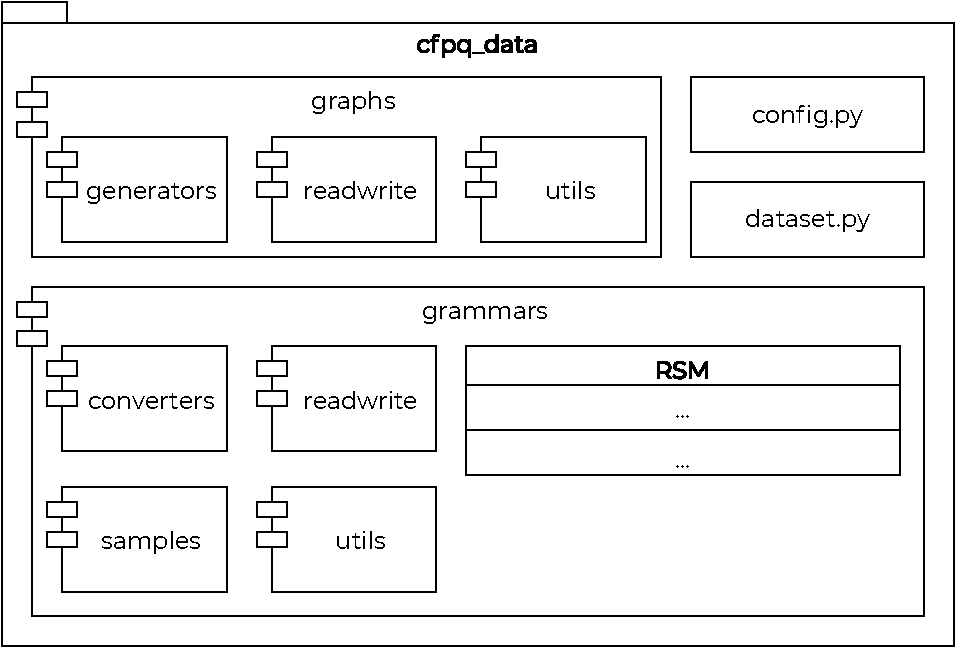
\includegraphics[width=\textwidth]{img/architecture_new.pdf}
    \caption{Новая архитектура \textsc{CFPQ\_Data}}
\end{figure}

Функции для манипулирования графами собраны в модуле <<graphs>>, который состоит из трех подмодулей.
\begin{itemize}
    \item В подмодуле <<generators>> реализованы функции генерации синтетических графов.
    \item В подмодуле <<readwrite>> реализованы функции чтения и записи графов, представленных в формате RDF и в формате троек <<вершина, метка ребра, вершина>>.
    \item В подмодуле <<utils>> реализованы функции для трансформации графов.
\end{itemize}

Функции для манипулирования грамматиками собраны в модуле <<grammars>>, который состоит из четырех подмодулей.
\begin{itemize}
    \item В подмодуле <<converters>> реализованы функции конвертации кон\-текстно-свобод\-ной грамматики между различными представлениями.
    \item В подмодуле <<readwrite>> реализованы функции чтения и записи кон\-текстно-свобод\-ной грамматики, представленной в различных форматах.
    \item В подмодуле <<samples>> реализованы примеры кон\-текстно-свобод\-ных запросов для соответствующих помеченных графов из <<graphs>>.
    \item В подмодуле <<utils>> реализованы функции для трансформации грамматик.
\end{itemize}

В файле <<dataset.py>> фиксируется информация о графах, сохраненных в \textsc{CFPQ\_Data}, соответствующая версии пакета, а в файле <<config.py>> фиксируется конфигурация доступа пакета к набору данных.

Также, с помощью GitHub Actions\footnote{GitHub Action интеграционного тестирования: \url{https://github.com/JetBrains-Research/CFPQ_Data/actions/workflows/tests.yml}, дата последнего доступа --- 04.06.2021} было реализовано интеграционное тестирование полученного пакета на юнит-тестах на различных операционных системах, с последующим сбором информации о покрытии кода.

\subsection{Документация}
Все предоставляемые пользователю функции были снабжены документацией, публикация которой добавлена в новой версии веб-сайта проекта.
Также на веб-сайт были добавлены следующие страницы.
\begin{itemize}
    \item Страница\footnote{<<Dataset>>: \url{https://jetbrains-research.github.io/CFPQ_Data/dataset/index.html}, дата последнего доступа --- 04.06.2021} с описанием графов из набора данных \textsc{CFPQ\_Data}.
    \item Страница\footnote{<<Install>>: \url{https://jetbrains-research.github.io/CFPQ_Data/install.html}, дата последнего доступа --- 04.06.2021} с руководством по установке пакета.
    \item Страница\footnote{<<Tutorial>>: \url{https://jetbrains-research.github.io/CFPQ_Data/tutorial.html}, дата последнего доступа --- 04.06.2021} с руководством помогающим начать пользоваться пакетом.
    \item Страница\footnote{<<Reference>>: \url{https://jetbrains-research.github.io/CFPQ_Data/reference/index.html}, дата последнего доступа --- 04.06.2021} с документацией всех функций, имеющихся в пакете.
    \item Страница\footnote{<<About>>: \url{https://jetbrains-research.github.io/CFPQ_Data/about.html}, дата последнего доступа --- 04.06.2021} с информацией о группе разработчиков проекта.
    \item Страница\footnote{<<License>>: \url{https://jetbrains-research.github.io/CFPQ_Data/license.html}, дата последнего доступа --- 04.06.2021} с лицензией проекта.
\end{itemize}

Также было сохранено индексирование проекта в Google Dataset Search и автоматизирована публикация сайта на GitHub Pages с помощью GitHub Actions\footnote{GitHub Action публикации веб-сайта: \url{https://github.com/JetBrains-Research/CFPQ_Data/actions/workflows/deploy_docs.yml}, дата последнего доступа --- 04.06.2021}.